\section{Linear Support Vector Regression}

In the case of regression the goal is to predict a real-valued output for $y'$ so that our training data is of the form:

\begin{equation}
	\{(x_i,y_i), x\in\Re^{m}, y_i\in\Re, i=1, \dots, n\} \label{eq:svr_data}
\end{equation}

The regression SVM use a loss function that not allocating a penalty if the predicted value $y'_i$ is less than a distance $\epsilon$ away from the actual value $y_i$, i.e., if $|y_i-y'_i| \leq \epsilon$, where $y'_i = w^T x_i + b$. The region bound by $y'_i\pm\epsilon \ \forall_i$ is called an $\epsilon$-insensitive tube. The output variables which are outside the tube are given one of two slack variable penalties depending on whether they lie above, $\xi^+$, or below, $\xi^-$, the tube, provided $\xi^+ \geq 0$ and $\xi^- \geq 0 \ \forall_i$:

\begin{equation} \label{eq:svr_consts}
	\begin{aligned}
		& y_i\leq y'_i+\epsilon+\xi^+ \ \forall_i \\
    	& y_i\geq y'_i-\epsilon-\xi^- \ \forall_i \\
    	& \xi_i^+, \xi_i^- \geq 0 \ \forall_i
	\end{aligned}
\end{equation}

The objective function for SVR can then be written as:

\begin{equation} \label{eq:quad_svr_obj}
    \begin{aligned}
        \min_{w,b,\xi^+,\xi^-} \quad & \frac{1}{2}\Vert w\Vert^{2} + C \sum_{i=1}^{n}(\xi_i^+ + \xi_i^-) \\
            \textrm{subject to} \quad & y_i - w^T x_i - b \leq \epsilon + \xi_i^+ \ \forall_i \\ & w^T x_i + b - y_i \leq \epsilon + \xi_i^- \ \forall_i \\ & \xi_i^+, \xi_i^- \geq 0 \ \forall_i
    \end{aligned}
\end{equation}

\begin{figure}[h!]
	\centering
  	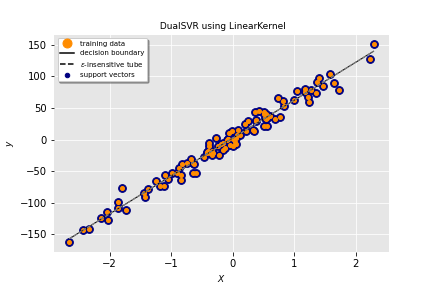
\includegraphics[scale=0.6]{img/linear_dual_svr_hyperplane.png}
  	\caption{Linear SVR hyperplane}
  	\label{fig:linear_dual_svr_hyperplane}
\end{figure}

\subsection{Epsilon-insensitive loss}

The \emph{epsilon-insensitive} loss is defined as:

\begin{equation} \label{eq:eps_loss1}
	\mathcal{L}_\epsilon = 
	\begin{cases}
		0 & \text{if } |y - (w^T x + b)| \leq \epsilon \\
		|y - (w^T x + b)| - \epsilon & \text{otherwise} \\
	\end{cases}
\end{equation}

or, equivalently:

\begin{equation} \label{eq:eps_loss2}
	\mathcal{L}_\epsilon = \max(0, |y - (w^T x + b)| - \epsilon)
\end{equation}

As the \emph{hinge} loss, also the \emph{epsilon-insensitive} loss is a nondifferentiable convex function due to its nonsmoothness in $\pm\epsilon$, but has a subgradient wrt $w$ that is given by:

\begin{equation} \label{eq:eps_loss_der}
	\frac{\partial \mathcal{L_\epsilon}}{\partial w}=
		\begin{cases}
            (y - (w^T x + b)) x & \text{if } |y - (w^T x + b)| > \epsilon \\
            0 & \text{otherwise} \\ 
        \end{cases}
\end{equation}

\subsubsection{Primal formulation}

The general primal unconstrained formulation takes the same form of \ref{eq:primal_svc}.

The quadratic optimization problem \ref{eq:quad_svr_obj} can be equivalently formulated as: 

\begin{equation} \label{eq:svr_eps}
	\min_{w,b} \frac{1}{2} \Vert w\Vert^{2} + C \sum_{i=1}^n \max(0, |y_i - (w^T x_i + b)| - \epsilon)
\end{equation}

where we make use of the \emph{epsilon-insensitive} loss \ref{eq:eps_loss1} or \ref{eq:eps_loss2}.

The above formulation penalizes slacks $\xi$ linearly and is called $\mathcal{L}_1$-SVR.

\begin{figure}[h!]
	\centering
  	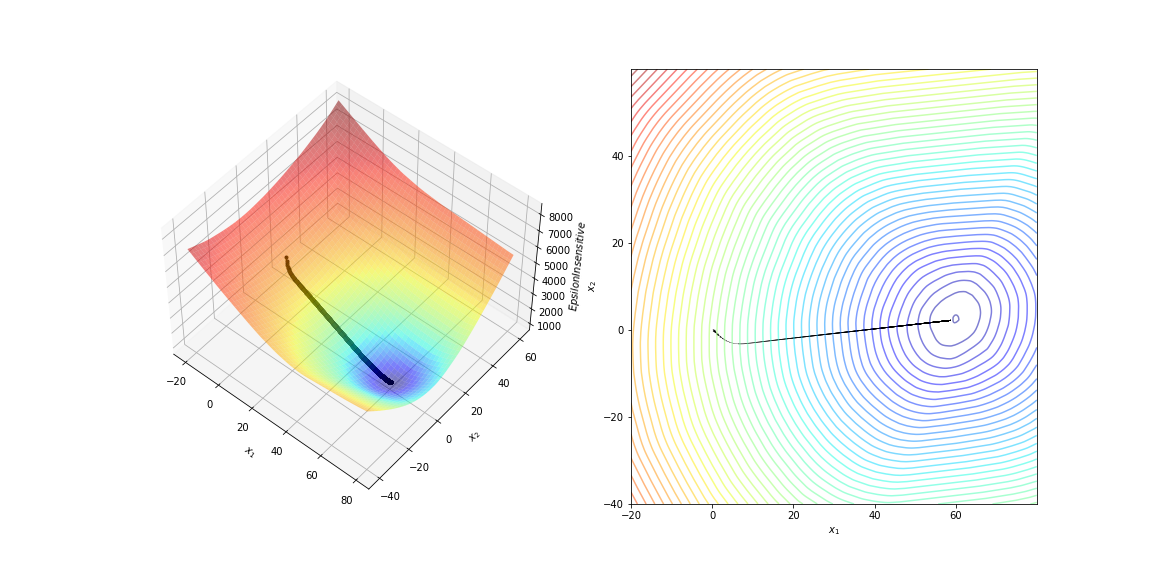
\includegraphics[scale=0.4]{img/svr_eps_loss.png}
  	\caption{SVR Epsilon-insensitive loss with optimization steps}
  	\label{fig:svr_eps_loss}
\end{figure}

\subsubsection{Wolfe Dual formulation}

To reformulate the \ref{eq:quad_svr_obj} as a \emph{Wolfe dual}, we introduce the Lagrange multipliers $\alpha_i^+ \geq 0, \alpha_i^- \geq 0, \mu_i^+ \geq 0, \mu_i^- \geq 0 \ \forall_i$:

\begin{equation} \label{eq:svr_wolfe_dual}
	\begin{aligned}
    	\max_{\alpha^+,\alpha^-,\mu^+,\mu^-} \min_{w,b,\xi^+,\xi^-} \mathcal{W}(w,b,\xi^+,\xi^-,\alpha^+,\alpha^-,\mu^+,\mu^-) = \frac{1}{2}\Vert w\Vert^{2}+C \sum_{i=1}^n(\xi_i^+ + \xi_i^-)-\sum_{i=1}^n(\mu_i^+ \xi_i^+ + \mu_i^- \xi_i^-) \\ -\sum_{i=1}^n\alpha_i^+(\epsilon+\xi_i^+ + y'_i-y_i)-\sum_{i=1}^n\alpha_i^-(\epsilon+\xi_i^- - y'_i+y_i)
	\end{aligned}
\end{equation}

Substituting for $y_i$, differentiating wrt $w, b, \xi^+$, $\xi^-$ and setting the derivatives to $0$ gives:

\begin{equation} \label{eq:svr_wolfe_der_w}
	\frac{\partial \mathcal{W}}{\partial w}=w-\sum_{i=1}^{n}(\alpha_i^+ - \alpha_i^-) x_i \Rightarrow w=\sum_{i=1}^{n}(\alpha_i^+ - \alpha_i^-) x_i
\end{equation}

\begin{equation} \label{eq:svr_wolfe_der_b}
	\frac{\partial \mathcal{W}}{\partial b}=-\sum_{i=1}^{n}(\alpha_i^+ - \alpha_i^-)\Rightarrow \sum_{i=1}^{n}(\alpha_i^+ - \alpha_i^-)=0
\end{equation}

\begin{equation}\label{eq:svr_wolfe_der_xip}
	\frac{\partial \mathcal{W}}{\partial\xi_i^+}=0\Rightarrow C=\alpha_i^+ + \mu_i^+
\end{equation}

\begin{equation} \label{eq:svr_wolfe_der_xim}
	\frac{\partial \mathcal{W}}{\partial\xi_i^-}=0\Rightarrow C=\alpha_i^- + \mu_i^-
\end{equation}

Substituting \ref{eq:svr_wolfe_der_w} and \ref{eq:svr_wolfe_der_b} in, we now need to maximize $\mathcal{W}$ wrt $\alpha_i^+$ and $\alpha_i^-$, where $\alpha_i^+ \geq 0,\ \alpha_i^- \geq 0 \ \forall_i$:

\begin{equation} \label{eq:svr_max_wolfe_dual}
    \max_{\alpha^+,\alpha^-} \mathcal{W}(\alpha^+,\alpha^-) = \sum_{i=1}^{n}y_i(\alpha_i^+ - \alpha_i^-)-\epsilon\sum_{i=1}^{n}(\alpha_i^+ + \alpha_i^-)-\frac{1}{2}\sum_{i,j}(\alpha_i^+ - \alpha_i^-)\langle x_i, x_j \rangle(\alpha_j ^+ - \alpha_j ^-)
\end{equation}

Using $\mu_i^+ \geq 0$ and $\mu_i^- \geq 0$ together with \ref{eq:svr_wolfe_der_w} and \ref{eq:svr_wolfe_der_b} means that $\alpha_i^+ \leq C$ and $\alpha_i^- \leq C$. We therefore need to find:

\begin{equation} \label{eq:svr_min_wolfe_dual}
    \begin{aligned}
        \min_{\alpha^+,\alpha^-} \quad & \frac{1}{2}(\alpha^+ - \alpha^-)^TK(\alpha^+ - \alpha^-)+\epsilon q^T(\alpha^+ + \alpha^-)-y^T(\alpha^+ - \alpha^-) \\
            \textrm{subject to} \quad & 0\leq\alpha_i^+,\alpha_i^- \leq C \ \forall_i \\ & q^T(\alpha^+ - \alpha^-)=0
    \end{aligned}
\end{equation}

where $q^T = [1, \dots, 1]$.

We can write the \ref{eq:svr_min_wolfe_dual} in a standard quadratic form as:

\begin{equation}
    \begin{aligned} \label{eq:svr_min_qp_wolfe_dual}
        \min_{\alpha} \quad & \frac{1}{2}\alpha^T Q\alpha-q^T\alpha \\
            \textrm{subject to} \quad & 0\leq\alpha_i\leq C \ \forall_i \\ & e^T\alpha=0
    \end{aligned}
\end{equation}

where the Hessian matrix $Q$ is 
$
\begin{bmatrix}
K & -K\\
-K & K 
\end{bmatrix}$
, $q$ is 
$
\begin{bmatrix}
-y\\
y
\end{bmatrix}$ + $\epsilon$
, and $e$ is 
$
\begin{bmatrix}
1\\
-1
\end{bmatrix}$.

Each new predictions $y'$ can be found using:

\begin{equation} \label{eq:svr_pred}
    y'= \sum_{i=1}^{n}(\alpha_i^+ - \alpha_i^-)\langle x_i, x' \rangle+b
\end{equation}

A set $S$ of support vectors $x_s$ can be created by finding the indices $i$ where $0\leq\alpha\leq C$ and $\xi_i^+=0$ or $\xi_i^-=0$.

This gives us:

\begin{equation} \label{eq:svr_b}
    b=y_s-\epsilon-\sum_{m\in S}(\alpha_m^+ -\alpha_m^-) \langle x_m, x_s \rangle
\end{equation}

As before it is better to average over all the indices $i$ in $S$:

\begin{equation} \label{eq:svr_b_avg}
    b=\frac{1}{N_s}\sum_{s\in S}y_s-\epsilon-\sum_{m \in S}(\alpha_m^+ - \alpha_m^-)\langle x_m, x_s \rangle
\end{equation}

From \ref{eq:svr_min_qp_wolfe_dual} we can notice that the equality constraint $e^T \alpha = 0$ arises form the stationarity condition $\partial_{{b}} \mathcal{W}=0$. So, again, for simplicity, we can again consider the bias term $b$ embedded into the weight vector. We report below the box-constrained dual formulation \cite{hsu2002simple} that arises from the primal \ref{eq:primal_svc_hinge1} or \ref{eq:primal_svc_hinge2} where the bias term $b$ is embedded into the weight vector $w$:

\begin{equation} \label{eq:svr_min_bcqp_wolf_dual}
    \begin{aligned}
        \min_{\alpha} \quad & \frac{1}{2} \alpha^T (Q + ee^T)\alpha+q^T\alpha \\
            \textrm{subject to} \quad & 0\leq\alpha_i\leq C \ \forall_i
    \end{aligned}
\end{equation}

\subsubsection{Lagrangian Dual formulation}

In order to relax the constraints in the \emph{Wolfe dual} formulation \ref{eq:svr_min_wolfe_dual} we define the problem as a \emph{Lagrangian dual} relaxation by embedding them into objective function, so we need to allocate the Lagrangian multipliers $\mu \geq 0, \lambda_+ \geq 0$, $\lambda_- \geq 0$:

\begin{equation} \label{eq:svr_lagrangian_dual}
	\begin{aligned}
		    \max_{\mu,\lambda_+,\lambda_-} \min_{\alpha} \mathcal{L}(\alpha,\mu,\lambda_+,\lambda_-) &= \frac{1}{2} \alpha^T Q\alpha+q^T\alpha - \mu^T (e^T \alpha) - \lambda_+^T (u - \alpha) - \lambda_-^T \alpha \\
    &= \frac{1}{2} \alpha^T Q\alpha + (q - \mu e + \lambda_+ - \lambda_-)^T \alpha - \lambda_+^T u
	\end{aligned}
\end{equation}

where the upper bound $u^T = [C, \dots, C]$.

Taking the derivative of the Lagrangian $\mathcal{L}$ wrt $\alpha$ and settings it to 0 gives:

\begin{equation} \label{eq:svr_lagrangian_der_a}
	\frac{\partial \mathcal{L}}{\partial \alpha}=0\Rightarrow Q \alpha + (q - \mu e + \lambda_+ - \lambda_-) = 0
\end{equation}

With $\alpha$ optimal solution of the linear system:

\begin{equation} \label{eq:svr_lagrangian_sol}
    Q \alpha = - (q - \mu e + \lambda_+ - \lambda_-)
\end{equation}

the gradient wrt $\mu$, $\lambda_+$ and $\lambda_-$ are:

\begin{equation} \label{eq:svr_lagrangian_der_mu}
	\frac{\partial \mathcal{L}}{\partial \mu}=-e \alpha
\end{equation}

\begin{equation} \label{eq:svr_lagrangian_der_lp}
	\frac{\partial \mathcal{L}}{\partial \lambda_+}=\alpha - u
\end{equation}

\begin{equation} \label{eq:svr_lagrangian_der_lm}
    \frac{\partial \mathcal{L}}{\partial \lambda_-}=-\alpha
\end{equation}

If the Hessian matrix Q is indefinite, i.e., the Lagrangian function is not strictly convex since it will be linear along the eigenvectors correspondent to the null eigenvalues, the Lagrangian dual relaxation will be nondifferentiable, so it will have infinite solutions and for each of them it will have a different subgradient. In order to compute the gradient, we will choose $\alpha$ in such a way as the one that minimizes the residue, i.e. the least-squares solution:

\begin{equation} \label{eq:svr_lagrangian_krylov_sol}
	\begin{aligned}
		\min_{\alpha \in K_n(Q, b)} \quad & \Vert Q \alpha - b \Vert \\ 
		\textrm{where} \quad & b = - (q - \mu e + \lambda_+ - \lambda_-)
	\end{aligned}
\end{equation}

Since we are dealing with a symmetric but indefinite linear system we will choose a well-known Krylov method that performs the Lanczos iterate, i.e., symmetric Arnoldi iterate, called \emph{minres}, i.e., symmetric \emph{gmres}, which computes the vector $\alpha$ that minimizes $\Vert Q \alpha - b \Vert$ among all vectors in $K_n(Q, b) = span(b, Qb, Q^2b, \dots, Q^{n-1}b)$.

\bigskip

From \ref{eq:svr_min_qp_wolfe_dual} we can notice that the equality constraint $e^T \alpha = 0$ arises form the stationarity condition $\partial_{{b}} \mathcal{W}=0$. So, again, for simplicity, we can again consider the bias term $b$ embedded into the weight vector. In this way the dimensionality of \ref{eq:svr_lagrangian_dual} is reduced of 1/3 by removing the multipliers $\mu$ which was allocated to control the equality constraint $e^T \alpha=0$, so we will end up solving exactly the problem \ref{eq:svr_min_bcqp_wolf_dual}.

\begin{equation} \label{eq:svr_bcqp_lagrangian_dual}
	\begin{aligned}
    	\max_{\lambda_+,\lambda_-} \min_{\alpha} \mathcal{L}(\alpha,\lambda_+,\lambda_-) &= \frac{1}{2} \alpha^T (Q + ee^T)\alpha+q^T\alpha - \lambda_+^T (u - \alpha) - \lambda_-^T \alpha \\
    &= \frac{1}{2} \alpha^T (Q + ee^T)\alpha + (q + \lambda_+ - \lambda_-)^T \alpha - \lambda_+^T u
	\end{aligned}
\end{equation}

where, again, the upper bound $u^T = [C, \dots, C]$.

Now, taking the derivative of the Lagrangian $\mathcal{L}$ wrt $\alpha$ and settings it to 0 gives:

\begin{equation} \label{eq:svr_bcqp_lagrangian_der_a}
	\frac{\partial \mathcal{L}}{\partial \alpha}=0\Rightarrow (Q + ee^T) \alpha + (q + \lambda_+ - \lambda_-) = 0
\end{equation}

With $\alpha$ optimal solution of the linear system:

\begin{equation} \label{eq:svr_bcqp_lagrangian_sol}
    (Q + ee^T) \alpha = - (q + \lambda_+ - \lambda_-)
\end{equation}

the gradient wrt $\lambda_+$ and $\lambda_-$ are:

\begin{equation} \label{eq:svr_bcqp_lagrangian_der_lp}
	\frac{\partial \mathcal{L}}{\partial \lambda_+}=\alpha - u
\end{equation}

\begin{equation} \label{eq:svr_bcqp_lagrangian_der_lm}
    \frac{\partial \mathcal{L}}{\partial \lambda_-}=-\alpha
\end{equation}

\subsection{Squared Epsilon-insensitive loss}

The \emph{squared epsilon-insensitive} loss is defined as:

\begin{equation} \label{eq:squared_eps_loss1}
	\mathcal{L}_\epsilon^2 = 
	\begin{cases}
		0 & \text{if } |y - (w^T x + b)| \leq \epsilon \\
		|y - (w^T x + b)|^2 - \epsilon & \text{otherwise} \\
	\end{cases}
\end{equation}

or, equivalently:

\begin{equation} \label{eq:squared_eps_loss2}
	\mathcal{L}_\epsilon^2 = \max(0, |y - (w^T x + b)| - \epsilon)^2
\end{equation}

As the \emph{squared hinge} loss, also the \emph{squared epsilon-insensitive} loss is a convex function and it has a gradient wrt $w$ that is given by:

\begin{equation} \label{eq:squared_eps_loss_der}
	\frac{\partial \mathcal{L}_\epsilon^2}{\partial w}=
		\begin{cases}
            2 ((y - (w^T x + b)) x) & \text{if } |y - (w^T x + b)| > \epsilon \\
            0 & \text{otherwise} \\ 
        \end{cases}
\end{equation}

\subsubsection{Primal formulation}

To provide a continuously differentiable function the optimization problem \ref{eq:svr_eps} can be formulated as: 

\begin{equation} \label{eq:svr_squared_eps}
    \min_{w,b} \frac{1}{2} \Vert w\Vert^{2} + C \sum_{i=1}^n \max(0, |y_i - (w^T x_i + b)| - \epsilon)^2
\end{equation}

where we make use of the \emph{squared epsilon-insensitive} loss that quadratically penalized slacks $\xi$ and is called $\mathcal{L}_2$-SVR.

\begin{figure}[h!]
	\centering
  	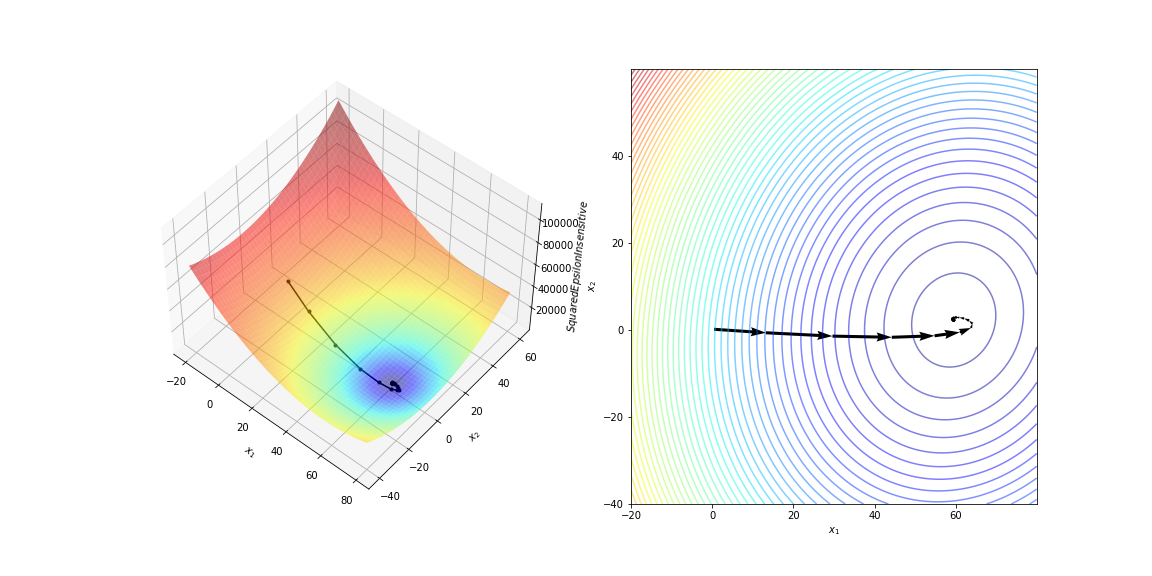
\includegraphics[scale=0.4]{img/svr_squared_eps_loss.png}
  	\caption{SVC Squared Epsilon-insensitive loss with optimization steps}
  	\label{fig:svr_squared_eps_loss}
\end{figure}
